\section{Addition Details on Algorithms}

\subsection{Asynchrony Through Warp Specialization for the Backward Pass}
\label{sec:algo_ws_bwd}

Similar to the forward pass~\cref{sec:algo_ws}, we use warp specialization to
handle asynchrony.
Instead of just a simple producer-consumer pattern in the forward pass, we add
one extra role of a $\vdQ$ writer, since we need to accumulate the value of $\vdQ$
produced by each thread block to the global value of $\vdQ$.
This $\vdQ$ accumulation introduces memory contention (many thread blocks writing to the same
location) so having a separate warp to handle this (along with asynchrony) will
avoid blocking the rest of the warps in the thread block to perform the next
computation (matmul).

We include the backward pass with warp specialization in~\cref{alg:flash3_wgmma_ws_bwd}.
\begin{algorithm}[H]
    \caption{\small\label{alg:flash3_wgmma_ws_bwd}\fat backward pass with warp specialization}
    \begin{algorithmic}[1]
\REQUIRE Matrices $\vQ, \vK, \vV, \vO, \vdO \in \mathbb{R}^{N \times d}$ in HBM,
logsumexp vector $L \in \mathbb{R}^N$ in HBM, block sizes $B_c$, $B_r$.
\STATE In a preprocessing kernel, compute $D = \mathrm{rowsum}(\vdO \circ \vO) \in \mathbb{R}^d$ (pointwise multiply), write
$D$ to HBM and divide it into $T_r$ blocks $D_1, \dots, D_{T_r}$ of size
$B_r$ each.
\STATE Divide $\vQ$ into $T_r = \left\lceil\frac{N}{B_r} \right\rceil$ blocks $\vQ_1, \dots, \vQ_{T_r}$ of size $B_r \times d$ each,
and divide $\vK, \vV$ in to $T_c = \left\lceil \frac{N}{B_c} \right\rceil$ blocks $\vK_1, \dots, \vK_{T_c}$ and
$\vV_1, \dots, \vV_{T_c}$, of size $B_c \times d$ each.
\STATE Divide $\vdO$ into $T_r$ blocks $\vdO_i, \dots, \vdO_{T_r}$
of size $B_r \times d$ each, and divide $L$ into $T_r$ blocks $L_i, \dots, L_{T_r}$ of size
$B_r$ each.
\STATE Initialize pipeline object to manage barrier synchronization with $s$-stage circular SMEM buffer.
\IF {in producer warpgroup}
\STATE Deallocate predetermined number of registers.
\STATE Issue load $\vK_j$ and $\vV_j$ from HBM to shared memory.
\STATE Upon completion, commit to notify consumer of the load of $\vK_j$ and $\vV_j$.
\FOR{$1 \le i \leq T_r$}
    \STATE Wait for the $(i\,\%\,s)$th stage of the buffer to be consumed.
    \STATE Issue loads of $\vQ_i, \vdO_i$ from HBM to shared memory at the $(i\,\%\,s)$th stage of the buffer.
    \STATE Upon completion, commit to notify consumers of the loads of $\vQ_i, \vdO_i$.
\ENDFOR
\ELSIF {in consumer warpgroups}
\STATE Reallocate predetermined number of registers as function of number of consumer warps.
\STATE On-chip, Initialize $\vdK_j = (0)_{B_c \times d}, \vdV_j = (0)_{B_c \times d}$ .
\STATE Wait for $\vK_j$ and $\vV_j$ to be loaded in shared memory.
\FOR{$1 \le i \leq T_r$}
\STATE Wait for $\vQ_i$ to be loaded in shared memory.
\STATE Load $L_i, D_i$ from HBM to on-chip SRAM.
\STATE On chip, compute $\vS_{i}^{(j)} = \vQ_i \vK_j^T \in \mathbb{R}^{B_r \times B_c}$
(SS-GEMM). Commit.
\STATE Wait for $\vdO_i$ to be loaded in shared memory.
\STATE On chip, compute $\vdP_{i}^{(j)} = \vdO_{i} \vV_j^\top \in \mathbb{R}^{B_r \times B_c}$
(SS-GEMM). Commit.
\STATE On chip, wait for $\vS_{i}^{(j)}$, then compute $\vP_{i}^{(j)} = \exp(\vS_{ij} - L_{i}) \in \mathbb{R}^{B_r \times B_c}$.
\STATE On chip, wait for $\vdP_i^{(j)}$, then compute $\vdS_{i}^{(j)} = \vP_{i}^{(j)} \circ (\vdP_{i}^{(j)} - D_i) \in \mathbb{R}^{B_r \times B_c}$.
\STATE On chip, compute
$\vdV_j \leftarrow \vdV_j + (\vP_{i}^{(j)})^\top \vdO_i \in \mathbb{R}^{B_c \times d}$ (RS-GEMM). Commit.
\STATE On chip, compute $\vdK_{j} \leftarrow \vdK_j + {\vdS_{i}^{(j)}}^\top \vQ_i \in \mathbb{R}^{B_c \times
  d}$ (RS-GEMM). Commit and wait for both $\vdV_j$ and $\vdK_j$.
\STATE On chip, compute $\vdQ_{i}^{(\mathrm{local})} = \vdS_{i}^{(j)} \vK_j \in
\mathbb{R}^{B_r \times d}$ (SS-GEMM), and write $\vdQ_i^{(\mathrm{local})}$ to smem. Notify
the $\vdQ$-writer.
\ENDFOR
\ELSIF{in $\vdQ$-writer warp}
\FOR{$1 \le i \leq T_r$}
\STATE Wait for $\vdQ_i^{(\mathrm{local})}$ to be ready in smem.
\STATE Using a semaphore, atomically add $\vdQ_i^{(\mathrm{local})}$ to $\vdQ_i$ in global memory.
\ENDFOR
\ENDIF
\end{algorithmic}
\end{algorithm}

\subsection{2-Stage Pipelining SASS Analysis}
\label{sec:2-stage-sass}

We give simplified SASS code for the inside of the consumer warpgroup mainloop.
\begin{small}
\begin{verbatim}
// Compute row_max
FMNMX.FTZ R0, R24, R6, !PT ;
SHFL.BFLY PT, R185, R2, 0x2, 0x1f ;
… FMNMX and SHFL.BFLY … 

// Apply exp2 and row_sum. Rescale O.
FMUL.FTZ R2, R4, UR9 ;
MUFU.EX2 R185, R184 ;                                            
FFMA.FTZ R24, R24, UR9, -R6.reuse ;
FADD.FTZ R24, R211, R24 ;                              
… FMUL, FFMA, FMUL, MUFU.EX2, FADD …

// FP32 -> FP16 conversion are interleaved with exp2, row_sum and O rescaling.
F2FP.F16.F32.PACK_AB R231, R25, R231 ;
… F2FP, FMUL, MUFU, FFMA, FADD ...

// Start the first WGMMA. Broken down into 8 HGMMAs.
// The first 7 HGMMAs are packed together.
WARPGROUP.ARRIVE ;
HGMMA.64x192x16.F32 R24, gdesc[UR44], RZ, !UPT ;
... HGMMA x 6 ...

// FP32->FP16, exp2, row_sum, O rescaling are interleaved with HGMMA. 
F2FP.F16.F32.PACK_AB R214, R214, R187 ; 
MUFU.EX2 R234, R5 ;
FADD.FTZ R237, R187, R2 ;
… F2FP, MUFU, FADD …

// The last HGMMA is issued here. No need to wait.
HGMMA.64x192x16.F32 R24, gdesc[UR44], R24, gsb0 ;

// Start the second WGMMA. Broken down into 12 HGMMAs.
// All 12 HGMMAs are packed together. Not interleaved with other instructions.
WARPGROUP.ARRIVE ;
HGMMA.64x128x16.F32 R120, R228, gdesc[UR8].tnspB, R120 ;
... HGMMA x 10 ...
HGMMA.64x128x16.F32 R120, R184, gdesc[UR8].tnspB, R120, gsb0 ;

// wgmma.wait_group at the end.
WARPGROUP.DEPBAR.LE gsb0, 0x0 ; 

\end{verbatim}
\end{small}

We make the following observations:
\begin{enumerate}
    \item Softmax is reordered to the very beginning, even before the first WGMMA. \TD{why?}
    \item The first WGMMA is interleaved with softmax and FP32 $\rightarrow$ FP16 datatype conversion of $\vS$. This indicates that WGMMA and non-WGMMAs are executed in parallel.
    \item \verb|exp2|, \verb|row\_sum|, O rescaling and FP32 $\rightarrow$ FP16 conversions are interleaved together. \TD{what's the benifit since these instructions are synced?} 
    \item The second WGMMA is not overlapped with other instructions, as expected.
\end{enumerate}
Overall, SASS shows that the 2-stage pipelining idea works as expected.

\subsection{3-Stage Pipelining Algorithm}
\label{sec:3-stage}
We experiment with a 3-stage pipelining algorithm to parallelize the first WGMMA from iteration $j+2$, softmax from iteration $j+1$, and the second WGMMA from iteration $j$. We describe this algorithm in \cref{alg:flash3_3_stage_wgmma}. 
This algorithm behaves worse than the 2-stage pipelining algorithm due to the reasons below:

\begin{figure}[ht]
    \centering
    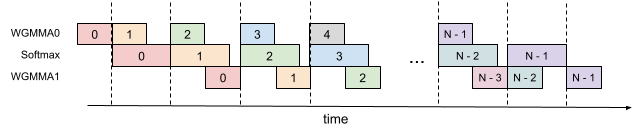
\includegraphics[width=.95\linewidth]{figs/3_stage_pipelining.png}
    \caption{3-Stage Pipelining}
    \label{fig:3_stage_pipelining}
\end{figure}

\begin{algorithm}[H]
    \caption{\small\label{alg:flash3_3_stage_wgmma}\sysnameone 3-stage pipelining consumer warpgroup forward pass}
    \begin{algorithmic}[1]
      \REQUIRE Matrices $\vQ, \vK, \vV \in \mathbb{R}^{N \times d}$ in HBM, block sizes $B_c$, $B_r$.
      Each warpgroup reads 1 block Qi of size $B_r \times d$, $T_c = \left\lceil \frac{N}{B_c} \right\rceil$ blocks $\vK_1, \dots, \vK_{T_c}$ and
      $\vV_1, \dots, \vV_{T_c}$ of size $B_c \times d$.
      Each warpgroup writes 1 output block $\vO_i$ of size $B_r \times d$, and 1 logsumexp block $L_i$ of size $B_r$.
      \STATE Initialization. Load $\vQ_i$ from HBM to on-chip SRAM.
      Initialize $\vO_{i}, \ell_{i}, m_{i}, scale\_o$.
      \STATE Wait for the producer warpgroup loading $\vK_0$ from HBM to on-chip SRAM.
      \STATE Compute $\vS = \vQ_i \vK_0^T$ using WGMMA. Commit and wait.
      \STATE Compute $m_{i}$, $\tilde{\vP}_{i}$, $\ell_{i}$, $scale\_o$ based on $\vS$.
      \STATE Wait for the producer warpgroup loading $\vK_1$ from HBM to on-chip SRAM.
      \STATE Compute $\vS = \vQ_i \vK_1^T$ using WGMMA. Commit and wait.
      \FOR{$2 \le j < T_c - 2$}
        \STATE Wait for the producer warpgroup loading $\vK_j$ from HBM to on-chip SRAM.
        \STATE Compute $\vS\_next = \vQ_i \vK_{j}^T$ using WGMMA. Commit but do not wait.
        \STATE Wait for the producer warpgroup loading $\vV_{j-2}$ from HBM to on-chip SRAM.
        \STATE Rescale $\vO_{i}$ based on $scale\_o$.
        \STATE Compute
        $\vO_{i} = \vO_{i} + \tilde{\vP}_{i} \vV_{j-2}$ using WGMMA. Commit but do not wait.
        \STATE Compute $m_{i}$, $\tilde{\vP}_{i}\_next$, $\ell_{i}$, $scale\_o$ based on $\vS$.
        \STATE Wait for all previous WGMMAs.
        \STATE Copy $\vS\_next$ to $\vS$.
        \STATE Copy $\tilde{\vP}_{i}\_next$ to $\tilde{\vP}_{i}$.
      \ENDFOR
      \STATE Wait for the producer warpgroup loading $\vV_{T_c-2}$ from HBM to on-chip SRAM.
      \STATE Rescale $\vO_{i}$ based on $scale\_o$.
      \STATE Compute
      $\vO_{i} = \vO_{i} + \tilde{\vP}_{i} \vV_{T_c-2}$ using WGMMA. Commit and wait.
      \STATE Compute $m_{i}$, $\tilde{\vP}_{i}$, $\ell_{i}$, $scale\_o$ based on $\vS$.
      \STATE Wait for the producer warpgroup loading $\vV_{T_c-1}$ from HBM to on-chip SRAM.
      \STATE Rescale $\vO_{i}$ based on $scale\_o$.
      \STATE Compute
      $\vO_{i} = \vO_{i} + \tilde{\vP}_{i} \vV_{T_c-1}$ using WGMMA. Commit and wait.
      \STATE Epilogue. Rescale $\vO_{i}$ based on $\ell_{i}$. Compute $L_{i}$ based on $\ell_{i}$ and $m_{i}$. Write $\vO_{i}$ and $L_{i}$ to HBM as the $i$-th block of $\vO$ and $L$.
    \end{algorithmic}
  \end{algorithm}

\paragraph{Overlapping.} 
We expected that softmax can be overlapped with (the first WGMMA + the second WGMMA). However, the compiler doesn't cooperate in this way.
SASS code shows that only the first WGMMA is overlapped with softmax, while the second WGMMA is not. It's not clear why the compiler chooses to reorder instructions in this way.

\paragraph{Register pressure.}
This algorithm requires more registers compared to the 2-stage pipelining algorithm. 
In theory, it needs to store an extra $\tilde{\vP}_{i}$ and $scale\_o$, which is of size $B_r \times B_c \times \text{sizeof}(\text{input\_data\_type}) + B_r \times \text{sizeof}(\text{float})$.
As a result, a smaller block size needs to be chosen.













